\begin{myprop}
	\kw{Si} deux droites sont perpendiculaires à une même troisième droite, \kw{alors} ces deux droites sont parallèles.
\end{myprop}


\begin{myex}
	\begin{multicols}{2}
		\kw{On sait que} $(d_1)$ et $(d_2)$ sont toutes deux perpendiculaires à $(D)$.\\
		\kw{Donc} $(d_1)$ et $(d_2)$ sont parallèles.
		
		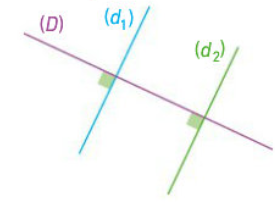
\includegraphics[scale=0.6]{img/para2}
	\end{multicols}
	
\end{myex}


\begin{myprop}
	\kw{Si} deux droites sont parallèles, \kw{alors} toute perpendiculaire à l’une est perpendiculaire à l’autre
\end{myprop}


\begin{myex}
	\begin{multicols}{2}
		\kw{On sait que} $(d_1)$ // $(d_2)$ et $(d_1) \perp (D)$\\
		\kw{Donc} $(d_2) \perp (D)$.
		
		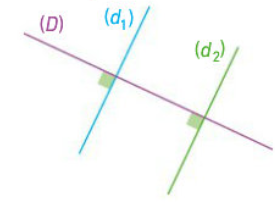
\includegraphics[scale=0.6]{img/para2}
	\end{multicols}
	
\end{myex}

\begin{myprop}
	\kw{Si} deux droites sont parallèles à une même troisième, \kw{alors} ces deux droites sont parallèles entre elles.
\end{myprop}

\begin{myex}
	\begin{multicols}{2}
		\kw{On sait que} $(d_1)$ // $(d)$ et $(d_2) // (d)$\\
		\kw{Donc} $(d_1) \perp (d_2)$.
		
		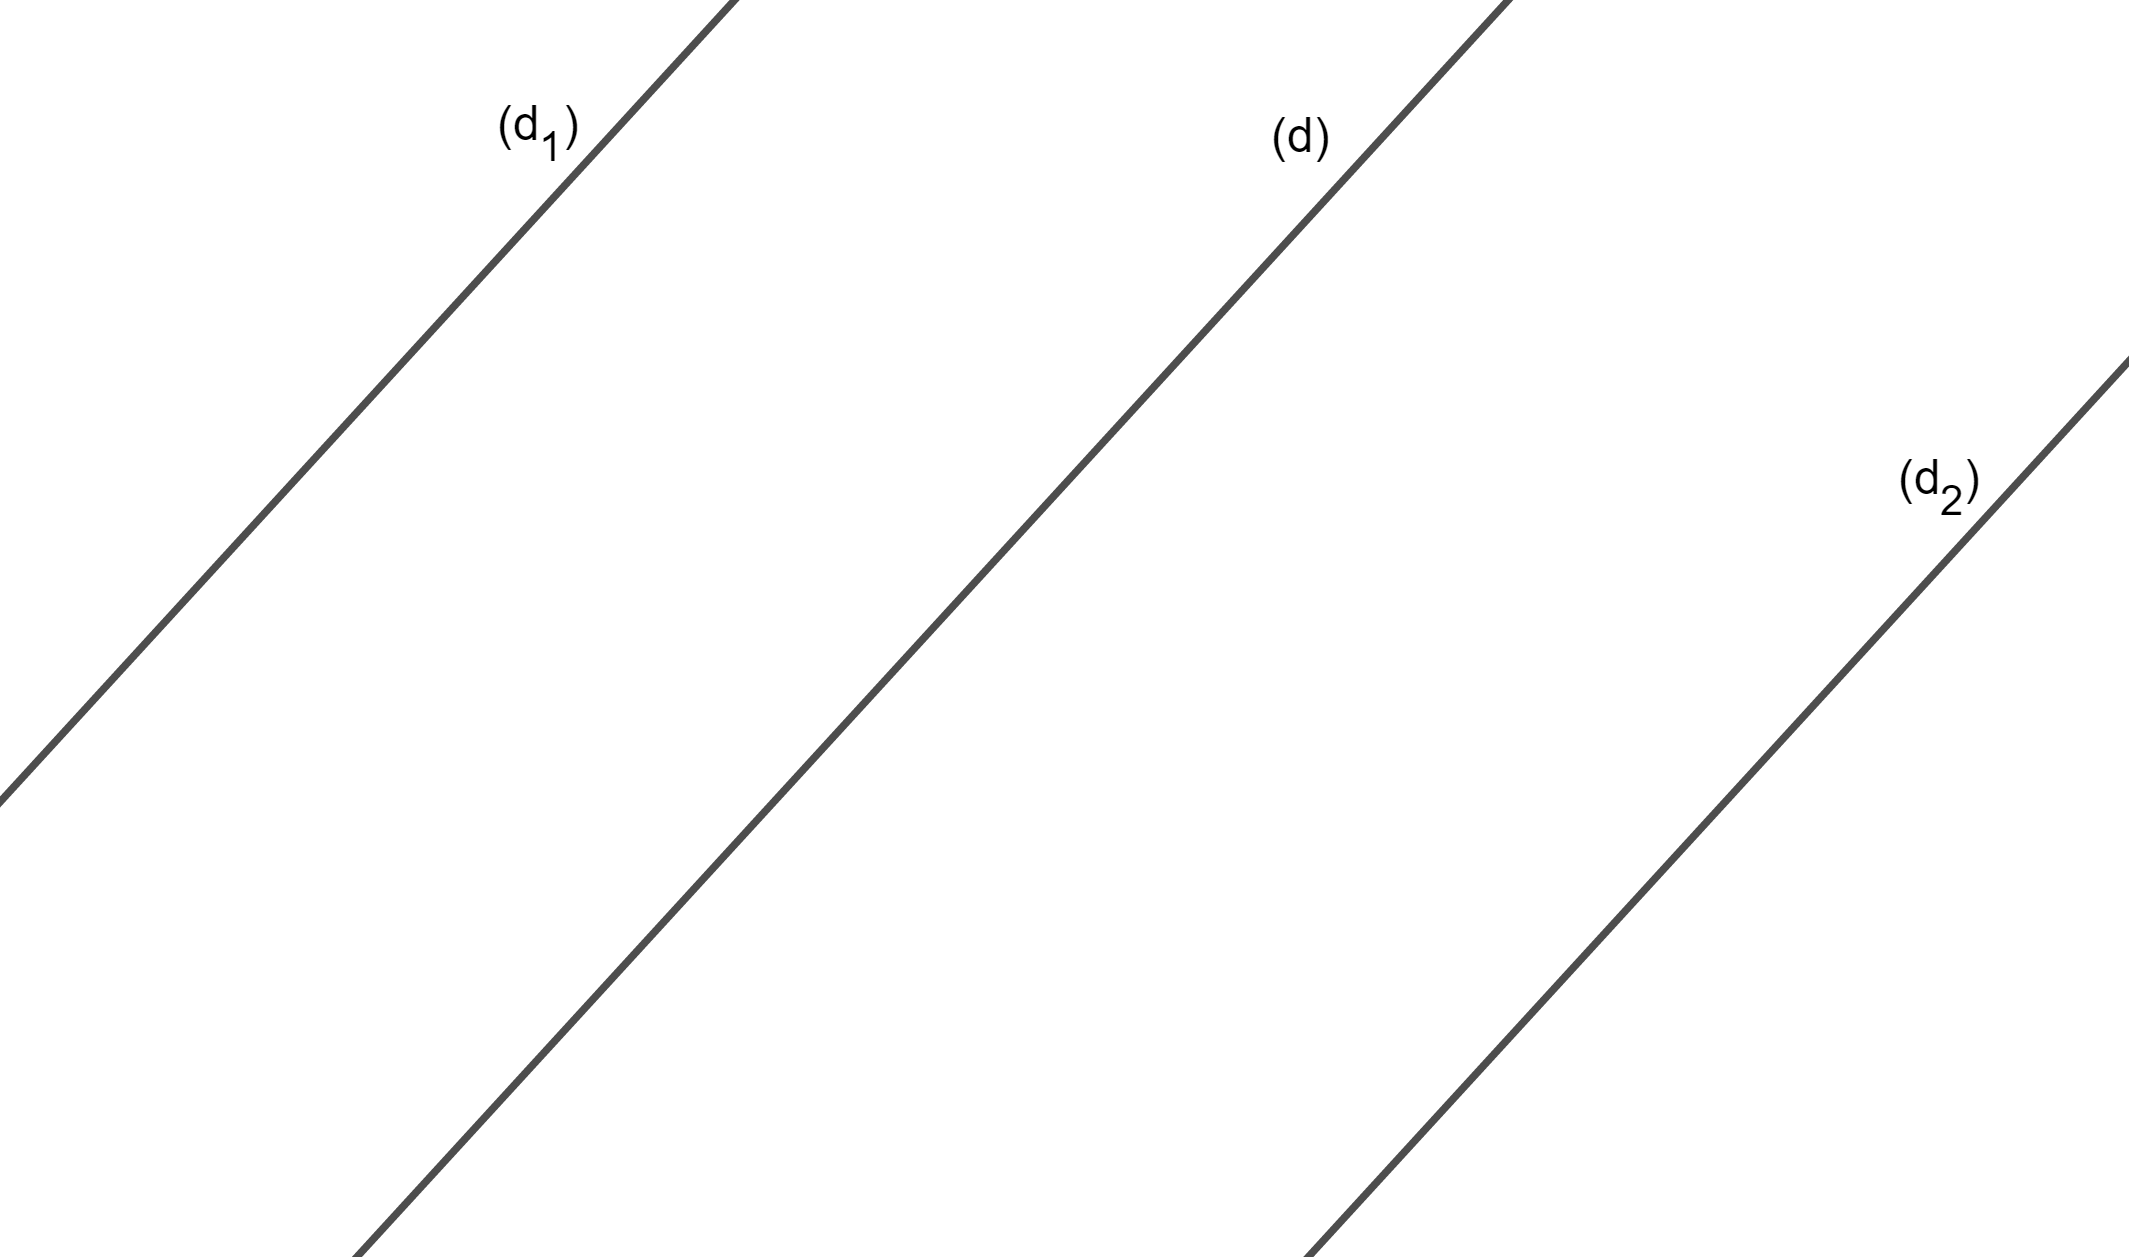
\includegraphics[scale=0.1]{img/para3}
	\end{multicols}
	
\end{myex}
